%%%%%%%%%%%%%%%%%%%%%%%%%%%%%%%%%%%%%%%%%%%%%%%%%%%%%%%%%%%%%%%%%%%%%%%%%%%%%%%%%%%%%%%%%%%%%%%%%%%%%%%%%%%%%%%%%%%%%%%%%%%%%%%%%%%%%%%%%%%%%%%%%%%%%%%%%%%
% This is just an example/guide for you to refer to when submitting manuscripts to Frontiers, it is not mandatory to use Frontiers .cls files nor frontiers.tex  %
% This will only generate the Manuscript, the final article will be typeset by Frontiers after acceptance.   
%                                              %
%                                                                                                                                                         %
% When submitting your files, remember to upload this *tex file, the pdf generated with it, the *bib file (if bibliography is not within the *tex) and all the figures.
%%%%%%%%%%%%%%%%%%%%%%%%%%%%%%%%%%%%%%%%%%%%%%%%%%%%%%%%%%%%%%%%%%%%%%%%%%%%%%%%%%%%%%%%%%%%%%%%%%%%%%%%%%%%%%%%%%%%%%%%%%%%%%%%%%%%%%%%%%%%%%%%%%%%%%%%%%%

%%% Version 3.4 Generated 2018/06/15 %%%
%%% You will need to have the following packages installed: datetime, fmtcount, etoolbox, fcprefix, which are normally inlcuded in WinEdt. %%%
%%% In http://www.ctan.org/ you can find the packages and how to install them, if necessary. %%%
%%%  NB logo1.jpg is required in the path in order to correctly compile front page header %%%

\documentclass[utf8]{frontiersSCNS} % for Science, Engineering and Humanities and Social Sciences articles
%\documentclass[utf8]{frontiersHLTH} % for Health articles
%\documentclass[utf8]{frontiersFPHY} % for Physics and Applied Mathematics and Statistics articles

%\setcitestyle{square} % for Physics and Applied Mathematics and Statistics articles
\usepackage{url,hyperref,lineno,microtype,subcaption}
\usepackage[onehalfspacing]{setspace}
\epstopdfsetup{outdir=./}

\linenumbers


% Leave a blank line between paragraphs instead of using \\


\def\keyFont{\fontsize{8}{11}\helveticabold }
\def\firstAuthorLast{Mrad {et~al.}} %use et al only if is more than 1 author
\def\Authors{Assaad Mrad\,$^{1,*}$, Mazen Nakad\,$^{1}$, Yanlan Liu\,$^{1}$ Jean-Christophe Domec\,$^{1,2}$, Sanna Sevanto\,$^{3}$ and Gabriel Katul\,$^{1,4}$}
% Affiliations should be keyed to the author's name with superscript numbers and be listed as follows: Laboratory, Institute, Department, Organization, City, State abbreviation (USA, Canada, Australia), and Country (without detailed address information such as city zip codes or street names).
% If one of the authors has a change of address, list the new address below the correspondence details using a superscript symbol and use the same symbol to indicate the author in the author list.
\def\Address{$^{1}$Nicholas School of the Environment, Duke University, Durham, NC, USA \\
$^{2}$ UMR INRA-ISPA 1391, Bordeaux Sciences Agro, Gradignan 33195, France \\
$^{3}$Earth and Environmental Sciences Division, Los Alamos National Laboratory, Los Alamos, New Mexico, USA \\
$^{4}$Department of Civil and Environmental Engineering, Duke University, Durham, NC}
% The Corresponding Author should be marked with an asterisk
% Provide the exact contact address (this time including street name and city zip code) and email of the corresponding author
\def\corrAuthor{Assaad Mrad}

\def\corrEmail{mradassaad2@gmail.com}




\begin{document}
\onecolumn
\firstpage{1}

\title[Dynamic optimality principle for water use strategies]{A dynamic optimality principle for water use strategies explains isohydric to anisohydric plant responses} 

\author[\firstAuthorLast ]{\Authors} %This field will be automatically populated
\address{} %This field will be automatically populated
\correspondance{} %This field will be automatically populated

\extraAuth{}% If there are more than 1 corresponding author, comment this line and uncomment the next one.
%\extraAuth{corresponding Author2 \\ Laboratory X2, Institute X2, Department X2, Organization X2, Street X2, City X2 , State XX2 (only USA, Canada and Australia), Zip Code2, X2 Country X2, email2@uni2.edu}


\maketitle


\begin{abstract}

%%% Leave the Abstract empty if your article does not require one, please see the Summary Table for full details.
\section{}
For full guidelines regarding your manuscript please refer to \href{http://www.frontiersin.org/about/AuthorGuidelines}{Author Guidelines}.

As a primary goal, the abstract should render the general significance and conceptual advance of the work clearly accessible to a broad readership. References should not be cited in the abstract. Leave the Abstract empty if your article does not require one, please see \href{http://www.frontiersin.org/about/AuthorGuidelines#SummaryTable}{Summary Table} for details according to article type. 


\tiny
 \keyFont{ \section{Keywords:} keyword, keyword, keyword, keyword, keyword, keyword, keyword, keyword} %All article types: you may provide up to 8 keywords; at least 5 are mandatory.
\end{abstract}

\section{Introduction}



In fact, multiple models grounded on stomatal optimization were put forward and tipped as accurate predictors of transpiration. The accuracy those predictions is crucial for climate forecasting. \textbf{Here offer summary of these models}.

While the assumption that stomatal opening trends are controlled by plant hydraulics is widely used in the plant community, there is a shortage of evidence corroborating this assumption. In this work, the effect of plant water use strategies (from conservative to aggressive) on stomatal conductance ($g$) and leaf water potential ($\psi_l$) is analyzed through a dynamical system perspective that allows setting multiple constraints. 

\citet{Manzoni2013} offer a similar dynamical system approach to the same phenomenon. Water use strategy is prescribed by assigning a 'carbon value' to the terminal soil moisture content around the rooting zone. This study is similarly framed with additional sub-daily measured forcings and constraints on water use such as neighboring tree competition. The results of this model are compared to actual measurements.

The work here answers the following question: to what degree does water use strategy (WUS) dictate stomatal control during dry-down? In a recent review of the theory of optimal stomatal control, \citet{Buckley2017} recognize the importance of delayed benefits such as keeping soil soil moisture at higher levels for future use. 

The goal here is not to develop a stomatal prediction package but to explore whether plant hydraulic traits alone are capable of placing stomatal behavior anywhere on the iso- or aniso-hydry spectrum. 

\section{Materials and Methods}

\subsection{Theory}

The principle adopted here is that plants maximize their carbon gain ($A$) over a drydown period. This principle assumes that plants freely control the stomatal conductance $g_s$ under constraints. Previous work constrained control of $g_s$ by enforcing instantaneous water balance at the soil level \citep{Manzoni2013}. To mathematically express this principle and constraint, an augmented Lagrangian is defined $L$:
\begin{equation}
    \label{eqn:Lagrangian}
    L\Big(g_s, x, \frac{dx}{dt}, \lambda, t\Big) = A(g_s, t) - \lambda \Bigg[ \frac{dx}{dt} - f_e\Big(g_s, x, \frac{dx}{dt}, t\Big)\Bigg],
\end{equation}
where $\lambda$ is the Lagrange multiplier in mol mol$^{-1}$, $x$ is the soil moisture, $t$ is time, and $f_e$ sums water inputs to the soil and subtracts outputs.

Because this principle states that $A$ is maximized over a drydown and not instantaneously, the objective function $J$ is the integral of $L$ from $t=0$ at the beginning of drydown to $t=T$ at the end of it:
\begin{equation}
    \label{eqn:Objective}
    J\Big(g_s, x, \frac{dx}{dt}, \lambda, t\Big) = \int_0^T L\Big(g_s, x, \frac{dx}{dt}, \lambda, t\Big).
\end{equation}

The goal then consists of finding the function of $g_s$ in terms of $t$ that maximizes $J$. This goal is achieved by solving the Euler-Lagrange equations using the method of the calculus of variations. A required step however is expressing $A$ and $f_e$ in terms of the control variable $g_s$ and the state variable $x$.

\subsection{Carbon gain}

The seminal work by \citet{Farquhar1980} expresses carbon assimilation, or biochemical demand of carbon $A_{demand}$, for a C3 leaf as either limited by the Rubisco enzyme activity under saturated incoming photosynthetically active radiation (PAR) or by ribulose-1,5-biphosphate (RuBP) activity under limiting incoming PAR. 
To avoid the use of non-differentiable functions and ad-hoc parameters, we adopt an accurate approximation of $A_{demand}$ developed elsewhere \citep{Vico2013}. $A_{demand}$ is approximated using a hyperbolic function:
\begin{equation}
    \label{eqn:vico_model}
    A_{demand} = k_1 \frac{c_i - \Gamma^*}{c_i + k_2},
\end{equation}
where $c_i$ is the carbon concentration inside the leaf. $k_1$ and $k_2$ are parameters determined by asymptotic limits imposed on $c_i$ described in \citet{Vico2013}. Namely, $k_1 = \frac{J}{4}$ and $k_2 = \frac{J}{4} \frac{a_2}{V_{c,max}}$. $\Gamma^*$ is the carbon compensation point which is the concentration of $c_i$ where carbon assimilation comes to a halt.

Equation \ref{eqn:vico_model} is of a Michaelis-Menten type where $k_1$ is interpreted as the maximum rate of carbon assimilation and $k_2$ prescribes the strength of carboxylation compared to oxygenation through $a_2$. Specifically, $a_2 = K_c (1+O_a/K_o)$ where $K_c$ and $K_o$ are Michaelis-Menten constants for CO$_2$ and O$_2$ respectively and $O_a$ is the atmospheric concentration of O$_2$.

The parameters of equation \ref{eqn:vico_model} ($V_{c,max}$, $\Gamma^*$, $K_c$, $K_o$) are temperature $T_a$ dependent while $J$ is both $T_a$ and PAR dependent \citep{Medlyn2002}. The dependence of $K_c$ and $K_o$ to $T_a$ is that of tobacco \citep{Bernacchi2001} and that of $\Gamma^*$ to $T_a$ is that of spinach reported elsewhere \citep{Brooks1985}. The dependence of $J$ and $V_{c,max}$ to $T_a$ is that of fertilized Pinus radiata \citep{Medlyn2002}.

The approximations used for $A_{demand}$ in equation \ref{eqn:vico_model} neglect: 1) the potential limitation by sucrose synthesis, 2) the contribution by dark respiration to $A_{demand}$, and 3) the temperature buffering effect of the leaf boundary layer such that leaf temperature is equal to atmospheric temperature $T_a$.

Furthermore, it is enforced that every CO$_2$ molecule captured from the atmosphere by the leaf is assimilated such that $A_{demand} = A_{supply}$. The supply of carbon from the atmosphere is modeled as a Fickian diffusion process through the stomatal opening:
\begin{equation}
    \label{eqn:supply}
    A_{supply} = g_s(c_a - c_i),
\end{equation}
where $c_a$ is the atmospheric concentration of CO$_2$.

Combining equations \ref{eqn:vico_model} and \ref{eqn:supply}, a formulation for $A$ in terms of $g_s$ that is explicitly independent from $c_i$ is obtained:
\begin{equation}
    \label{eqn:A_noci}
    A = \frac{1}{2}[k_1 + g_s(k_2 + c_a) - \sigma],
\end{equation}
where $\sigma = \sqrt{[(k_2 + c_a)g_s + k_1]^2 + 4k_1 g_s (\Gamma^*-c_a)}$

To sum up, if changes of $T_a$ and PAR with time are given, as well as $c_a$ and $O_a$, then $g_s$ is the only independent variable in equation \ref{eqn:A_noci}.

\subsection{Soil water balance}

% The ensure the continuity of the water stream throughout the tree, we model three vertically connected layers: the soil, the trunk and branches, and the leaves. Each of these layers are characterized by a hydraulic resistance that is non-linearly related to water potential. Prescribing hydraulic resistances to these different layers allows computation of quantities regarded as indicative of isohydric to anisohydric behaviour. Such quantities include leaf water potential ($\psi_l$) and stomatal conductance ($g_s$).

At the soil, we model the water budget as follows \citep{Rodriguez-Iturbe2007}:
\begin{equation}
    \label{eqn:soil_water}
    \frac{dx(t)}{dt} = f_e\Big(g_s, x, \frac{dx}{dt}, t\Big) = \frac{\nu}{ n Z_r}[- E(g_s, t) - U(x, t)],
\end{equation}
where $x(t)$ is the relative soil moisture in m$^3$ m$^{-3}$, $U$ are uncontrolled losses (independent of the plant) in mmol m$^{-2}$ s$^{-1}$, and E is the evapotranspiration rate from the plant in mmol m$^{-2}$ s$^{-1}$. Water fluxes are expressed per unit leaf area. $n$ is the soil porosity in m$^3$ m$^{-3}$ and $Z_r$ is the effective plant rooting depth in $m$. To ensure dimensional equivalence we multiply the right hand side by $\nu = \text{LAI} \, M_w/ \rho_w$. LAI is the leaf area index in m$^3$ m$^{-3}$, $M_w = 18 * 10^{-6}$ kg mmol$^{-1}$ is the molar weight of water, and $\rho_w = 1000$ kg m$^{-3}$ is its density. $U$ may account for both soil leakage away from the rooting zone and competition from other plant roots. $f_e$ was previously introduced in equation \ref{eqn:Lagrangian}. Missing in equation \ref{eqn:soil_water} is the rainfall input and this is because we are only considering drydown periods in this work. 

Soil leakage is modeled as free drainage such that water losses from leakage per unit soil area and per unit depth is equal to the soil conductivity $g_x$: \citep{campbell1974}:
\begin{equation}
    \label{eqn:soil_cond}
    g_x = g_{x,sat}x^{2b+3}.
\end{equation}
$g_{x,sat}$ is the soil conductivity at saturation and $b$ is the non-linearity parameter. Both of these parameters depend on soil type \citep{Clapp1978}. From the soil moisture, one could also compute the soil water potential ($\psi_x$):
\begin{equation}
    \label{eqn:Clapp_pot}
    \psi_x = \psi_{x,sat}x^{-b},
\end{equation}
where $\psi_{x,sat}$ is the soil water potential at saturation.

The soil to root conductance $g_{sr}$ is assumed to be the conductivity of the soil $g_x$ divided by the distance between soil and root $l_{sr}$. $l_{sr} = \sqrt{d_r Z_r \text{RAI}}$ where $d_r$ is the fine root diameter in m and RAI is the root area index \citep{Manzoni2013}. If $g_x$ is given in kg s m$^{-3}$, then
\begin{equation}
    \label{eqn:soil_root}
    g_{sr} = \frac{10^9}{M_w \, \rho_w \, l_{sr} \, \text{LAI}} g_x, 
\end{equation}
where $g_{sr}$ has units of mmol m$^{-2}$ MPa$^{-1}$ s$^{-1}$ and is expressed per unit leaf area. Because the soil to root distance is taken into account in $g_{sr}$, one only needs to multiply $g_{sr}$ by the water potential difference between root and soil to get the volume flux of water.
\subsection{Leaf-level water balance}

As a point of departure from previous analyses based on the carbon gain maximization principle, it is recognized that plant transpiration is limited by the the plant hydraulic architecture when atmospheric water demand exceeds potential supply. This limitation imposes an upper bound on $g_s$. 

The loss of conductivity function of the whole plant with respect to water potential is known as a vulnerability curve (VC). We approximate the VC of the whole hydraulic pathway (roots, trunk, and branches) with a Weibull exceedance function such that:
\begin{equation}
    \label{eqn:root_leaf}
    g_{rl} = g_{rl,max}exp\Big[-\Big(\frac{\psi}{\psi_{63}}\Big)^s\Big],
\end{equation}
where $g_{rl}$ is the root to leaf hydraulic conductance in mmol m$^{-2}$ MPa$^{-1}$ s$^{-1}$ expressed per unit leaf area, and $g_{rl,max}$ is its maximum value at saturation. $\psi_{63}$ is the water potential at which the plant loses about 63\% of its conductance. Finally, $s$ controls the slope of the Weibull function at $\psi_{63}$ and therefore its curvature. 
% To find $\psi_{p}$, we invoke the hydrostatic approximation between leaves and roots which leads to $\psi_{p}=\frac{\psi{r}+\psi_l}{2}$ where $\psi_r$ is the root water potential.

We can now express $E$ at the soil, plant, and leaf levels as follows:
\begin{equation}
    \label{eqn: mass_cons}
        \begin{split}
        E & = E_{demand} = 1.6\: \text{LAI }\, g_s\, \text{VPD} \\
        & = E_{sr} = g_{sr}(\psi_x)*(\psi_x - \psi_r)\\
        & = E_{rl} = \int_{\psi_r}^{\psi_l} g_{rl}(\psi) d\psi \\
        \end{split}
\end{equation}
$E_{demand}$ is the atmospheric demand of water, $E_{sr}$ is the soil to root water supply, $E_{rl}$ is the root to leaf supply. All expressions of $E$ are given in units of mmol m$^{-2}$ s$^{-1}$ expressed per unit leaf area. The $E_{rl}$ expression is analogous to porous media methods where it is recognized that water potential is not distributed uniformly along the medium. This expression was also introduced elsewhere in plant science \citep{Sperry2017} and will allow for easier model comparison.

It is noted that as $g_s$ varies with time, $\psi_l$ also varies to match supply and demand. The hydraulic constraint from plant water supply is apparent when one realizes that while $E_{demand}$ is always increasing with $g_s$ for constant VPD, water supply through $E_{sr}$ and $E_{rl}$ have maxima that cannot be exceeded due to the decrease of hydraulic conductance functions $g_{sr}$ and $g_{rl}$ with increasing $\psi_x$, $\psi_r$, and $\psi_l$ (equations \ref{eqn:soil_root}, \ref{eqn:root_leaf}, and \ref{eqn: mass_cons}). The presence of a maximum possible water supply imposes an additional constraint on the stomatal conductance $g_s$. 

This additional constraint could be imposed with the help of another Lagrange multiplier. However, to maintain familiarity with the traditional definition of the marginal water use efficiency \citep{cowan1977}, this additional constraint is imposed differently here. Specifically, if maximizing $J$ (equation \ref{eqn:Objective}) leads to a $g_s$ that exceeds the maximum achievable $E$ at current $x$, then this $g_s$ is replaced artificially by finding the maximum transpiration rate \Big(at $\frac{\partial E}{\partial \psi_l} = 0$\Big). This rests on the assumption that plants take full advantage of their transpiration capacity.

\subsection{Maximizing the objective}

To maximize $J$ (equation \ref{eqn:Objective}), we use the method of the calculus of variations \citep{witelski2015} to derive what are known as the Euler-Lagrange equations (see equation 3.55 in the mentioned reference). For this problem, these are a set of three equations to be solved with two boundary conditions set on $x$ at the beginning of drydown $t=0$ and at the end of it $t=T$.

The control equation,
\begin{equation}
    \label{eqn:control}
    \frac{\partial L}{\partial g_s} = \frac{\partial A}{\partial g_s} + \lambda \frac{\partial f_e}{\partial g_s} = 0,
\end{equation}
gives a monotonic inverse relation between $\lambda$ and $g_s$ (see Results).

The co-state equation is $\frac{\partial L}{\partial x} - \frac{d}{dt} \Big(\frac{\partial L}{\partial x'} \Big) = 0$, where $x'= \frac{dx}{dt}$. The co-state equation yields the time variation of $\lambda$,
\begin{equation}
    \label{eqn:co_state}
    \frac{d \lambda}{dt} = \frac{\partial A}{\partial x} + \lambda \frac{\partial f_e}{\partial x} = \lambda \frac{\partial U}{\partial x}.
\end{equation}

Finally, the sate equation, $\frac{\partial L}{\partial \lambda} = 0$ gives the soil water balance (equation \ref{eqn:soil_water}). 

Of equal importance are the boundary conditions: equations \ref{eqn:control}, \ref{eqn:co_state}, and \ref{eqn:soil_water} are to be solved with preset initial and terminal soil moisture:
\begin{equation}
    \label{eqn: BC_no_WUS}
    \begin{split}
        BC_1 &:x(0)\\
        BC_2 &:x(T)\\
    \end{split}
\end{equation}
In reality, it is impossible to set the terminal soil moisture a priori. However, this can be mended by introducing the water use strategy (WUS).

\subsection{Water use strategy (WUS)}

To avoid having to set $x(T)$ a priori, we add a terminal gain term to $J$. The objective function $J$ in this situation is the following:
\begin{equation}
    \label{eqn:objective}
    J_{WUS} = \int_0^{T_f} L\Big(g_s, x, \frac{dx}{dt},\lambda,t \Big) dt + J_{T},
\end{equation}
where $J_{T}$ is the carbon value of the terminal soil water moisture $x(T)$ prescribed as:
\begin{equation}
    \label{eqn:terminal_gain}
    J_{T} = \Lambda x(T),
\end{equation}
where $\Lambda$ is a user-defined parameter, in mol mol$^{-1}$. Deriving the Euler-Lagrange equations once more to maximize $J_{WUS}$ gives the same differential equations (equations \ref{eqn:soil_water}, \ref{eqn:control}, \ref{eqn:co_state}) but with the main difference that the boundary condition at time $T$ is now set on $\lambda$: 
\begin{equation}
\label{eqn: BC_WUS}
    \begin{split}
        BC_1 &:x(0)\\
        BC_2 &:\lambda(T) = \Lambda.\\
    \end{split}
\end{equation}

Prescribing large $\Lambda$ corresponds to a conservative WUS and an aggressive WUS when it is small. This approach departs from the assumption that carbon gain trends are instantaneously optimal for all plants because residual soil moisture at the end of dry-down now has carbon value. The presence of $J_{T}$ in equation \ref{eqn:objective} represents in opportunity cost, measured in carbon gain units, of depleting the soil of water and increasing cavitation on the short term.

By tweaking the prescribed vulnerability curve for the same long-term strategy ($\Lambda$), and vice versa, it is possible to discern their effect on optimal stomatal behavior. 

\subsection{Environmental data} 

The model requires supplying environmental data acting as boundary conditions at the soil and leaf levels. These are the initial soil water content ($x_0$), vapor pressure deficit (VPD), incident leaf shortwave radiation ($R_l$), and temperature ($T$). We use the data provided by the FLUXNET project at the Blodgett forest. A drydown period starting on May 29, 2005 was chosen and the environmental variations over 20 days are averaged into one representative day. These conditions are then copied and tiled to however many days the optimization is running for. This allows isolating plant hydraulics and WUS.

The work here neglects high-frequency (sub-minute time scale) changes in environmental variables such as temperature and wind as well as those happening over multiple months such as changes in leaf nitrogen. The are thought not to have an appreciable effect on stomatal control over the timescale of a few weeks that is considered.

\section{Results}

\subsection{Demand driven transpiration}

Equation \ref{eqn:control} provides a complex functional dependence between $g_s$, $\lambda$, and environmental variables \citep{Katul2009a}:
\begin{equation}
    \label{eqn:gs_vs_env_lambda}
    \begin{split}
        g_s = & - \frac{k_1 (k_2-c_a+2 c_p)}{(k_2+c_a)^2} \\
        & +\frac{\sqrt{a\, \text{VPD}\, \lambda\, k_1^2 (c_a-c_p)(k_2+c_p)(k_2+c_a-2 a\, \text{VPD}\, \lambda)^2(k_2+c_a-a\, \text{VPD}\, \lambda)}}{a\, \text{VPD}\, \lambda (k_2+c_a)^2(k_2+c_a-a\, \text{VPD}\, \lambda)} ,
    \end{split}
\end{equation}
where $g_s$ is per leaf area. By far, the most influential atmospheric variable is VPD. The $g_s$ vs $\lambda$ phase space is therefore plotted for multiple VPD values (figure \ref{fig:gs_E_lam}a). $T_a$ and PAR and therefore $k_1$, $k_2$, and $c_p$, are set to their noon values (figure \ref{fig:environment}).

While this phase space is static in terms of $T_a$ and PAR, the dynamics of $g_s$ in response $\lambda$ and VPD shown stay the same. In the case where water supply is not limited through the rhizosphere or the plant water pathway (equations \ref{eqn:soil_root}, \ref{eqn:root_leaf}), $g_s$ decreases as the air dries (as VPD increases) and vice versa for constant $\lambda$. This vertical trajectory of $g_s$ closely resembles what would happen on a sub-daily timescale when $\lambda$ doesn't change appreciably due to lack of time. This is one driver of the midday stomatal closure when VPD is higher.

Another reason for a constant $\lambda$ could be the absence of uncontrolled losses $U$ (equation \ref{eqn:co_state}). If competitive water sinks such as other plants or leakage exist, and the day to day change in VPD is absent, then $g_s$ also decreases due to an increase in $\lambda$. This $g_s$ decrease is more noticeable at larger time scales of around 24 hours to allow $\lambda$ to change significantly. Realistically, droughts are accompanied with progressively drier air such that the combination of an increase of day to day VPD and an increase in $\lambda$ lead to a steeper decline in $g_s$ compared to the isolated action of these two effects.

 Another cause for an increase in $\lambda$ following this solid arrow is an increasingly supply-limited transpiration stream through the rhizosphere and the plant (an increase in PLC; equation \ref{eqn:supply}). This is seen by noticing that the solid arrow has a strong component normal to the lines of constant transpiration represented by red dashed lines in figure \ref{fig:gs_lam}. If however the changes in VPD are faster that changes in PLC then $g_s$ and $\lambda$ dynamics follow the short-dashed two-sided arrow that follows transpiration isolines. 

Figure \ref{fig:gs_lam} elucidates how transpiration demand through VPD and supply through the PLC can drive the midday stomatal closure. For a demand-driven transpiration stream and a constant $\lambda=12$ mmol mol$^{-1}$, a VPD$=8$ mmol mol$^{-1}$ corresponds to a $g_s\approx 40$ mol m$^{-2}$ s$^{-1}$ for the environmental conditions depicted in the caption of the mentioned figure. If at midday the VPD doubles, $g_s$ becomes 0 indicating a full stomatal closure. If however, $\lambda=5$ mmol mol$^{-1}$, then for the same VPD change $g_s$ goes from $\approx 81$ mol m$^{-2}$ s$^{-1}$ to $\approx 43$ mol m$^{-2}$ s$^{-1}$, a noticeable but less aggressive decrease in $g_s$ ($\approx 48\%$). However, a larger PAR and $T_a$ could buffer that decrease by accelerating the chemical reactions visible through increases in $k_1$ and $k_2$.

\subsection{Supply limited transpiration}

Supply limited transpiration occurs when the plant water pathway is inhibited enough by cavitation to set upper limits on $E$. This upper limit is called $E_{max}$ and defines the maximizing $g_s$, $\psi_r$, and $\psi_l$ at different $\psi_x$ (figure \ref{fig:gmax_Emax_psix}b,c). Figure \ref{fig:gmax_Emax_psix}a shows the partitioning of the total soil-root-leaf conductance into its soil-root and root-leaf components. Three VCs are compared in figure \ref{fig:gmax_Emax_psix} and they represent a resistant plant when $\psi_{63} = -3$ MPa, $s=4$, and $g_{rl,max} = 2$ mmol m$^{-2}$ MPa$^{-1}$ s$^{-1}$, a vulnerable plant when $\psi_{63} = -1.5$ MPa, $s=4$, and $g_{rl,max} = 2$ mmol m$^{-2}$ MPa$^{-1}$ s$^{-1}$, and an exponential plant when $\psi_{63} = -1$ MPa, $s=1$, and $g_{rl,max} = 8$ mmol m$^{-2}$ MPa$^{-1}$ s$^{-1}$. These three plant will be the same used in future comparisons throughout this work.



Supply limited midday stomatal closures are more nuances because they also lead to variations in $\lambda$ that could be positive or negative as seen by following transpiration isolines (red dashed lines in figure \ref{fig:gs_lam}). These isolines are considered a liberal path for the decrease in $g_s$ as the air dries in supply-limited conditions because PLC is also likely to increase as water is being used up by the plant. One can therefore expect a steeper decrease in $g_s$ as the air dries.

\subsection{Sensitivity of stomatal conductance to drying soil}

As previously described, root-to-leaf plant hydraulics are prescribed through a Vulnerability Curve (VC). By setting an upper limit on $E$ and therefore $g_s$, the VC sets a lower limit on the value of the marginal use efficiency $\lambda$ (figure \ref{fig:lam_lower}) because of the inverse relation between $g_s$ and $\lambda$ (equation \ref{eqn:control}). An upper limit on $\lambda$ is set at $g_s=0$ because $g_s$ cannot be negative (equation \ref{eqn:control}). As the soil moisture decreases and the soil water potential gets more negative, the leaf is constrained to higher $\lambda$ while the upper limit maintains a constant value. A more stringent lower limit applies when the plant is more vulnerable to embolism spread as indicated by a lower $\psi_{63}$. That vulnerable plants are constrained to more efficient modes of water use means that they can only afford more conservative water use strategies (WUS) as will be discussed.



This phenomenon is further shown in a simulation where plants use soil water over a period of $T=10$ days (figures \ref{fig:resistant_vulnerable_gs} and \ref{fig:resistant_vulnerable_lambda}). The soil water potential is preset by the boundary conditions to decrease from $x(0)=0.2$ to $x(T)=0.15$. There is no competition in this simulation to isolate plant water use from all possible effects. The half-hourly dynamics of $g_s$ show that the resistant plant ($\psi_{63}=3$) MPa maintain the same trend day to day. This is both due to the highly resistant xylem and the fact that environmental conditions are repeated day to day (figure \ref{fig:environment}). In contrast, the vulnerable plant ($\psi_{63}=1.9$) MPa starts at $t=0$ days with higher stomatal conductance than its resistant counterpart and progressively reduces its half-hour $g_s$ trend day to day. The contrast is clear when comparing the midday $g_s$ values against $t$ (figure \ref{fig:resistant_vulnerable_gs}a) and against $\psi_x$ (\ref{fig:resistant_vulnerable_gs}b). The larger sensitivity of the vulnerable plant's $g_s$ to $\psi_x$ qualify it as an isohydric species while the absent sensitivity of the resistant plant qualify it as an anisohydric species \citep{Hochberg2017}. As an intermediate case, the midrange species ($\psi_{63}=2.2$) MPa transitions from isohydric behavior when $\psi_x>-0.4$ MPa to anisohydric behavior.

This contrast in behavior is driven solely by plant hydraulics (figure \ref{fig:resistant_vulnerable_lambda}). As the soil dries and $\lambda_{lower}$ increases, it crosses the half-hourly trend in $\lambda$ for the 3 species shown but earlier for more vulnerable ones (higher $\psi_{63}$). During the crossing intervals, plant hydraulics, as limited by the VCs, drive plant water use and induces the sensitivity of $g_s$ to drying soil. Because this crossing happens earlier for the vulnerable plant, it has to resort to more aggressive water use (lower $\lambda$) to achieve the same water use as prescribed by the boundary conditions. This underscores the disadvantage of having to prescribe the initial and terminal soil moisture as boundary conditions as priori. If the resistant plant can afford to be more aggressive and be more competitive than the vulnerable plant in the same environment, then a different formulation that take WUS into account is warranted. In fact, the total carbon assimilation over the 10-day period for the resistant plant is 3.10 mol m$^{-2}$ compared to 3.02 mol m$^{-2}$ for the vulnerable plant indicating a negligible competitive advantage. This is also apparent comparing the PLC at $t=10$ days of the resistant plant of 81\% compared to the vulnerable plant's 83\%. The widely used Hamiltonian integrates both carbon assimilation and the carbon cost of using water (Appendix B):
\begin{equation}
    \label{eqn:Hamiltionian}
    H = A + \lambda f_e.
\end{equation}
For the resistant plant , the integral of the Hamiltonian over the 10-day period is 0.78 mol m$^{-2}$ whereas it is 0.80 mol m$^{-2}$, a negligible difference. However, if one equates the amount of time above a certain threshold PLC to plant water stress, then one would be interested in observing that the vulnerable plant spends 8 days above a PLC$=50\%$ compared to the resistant plant's 2 days (figure S1).

A terminal gain term that is proportional to the terminal soil moisture $x(T)$ is now used in the objective (equation \ref{eqn:terminal_gain}). The boundary conditions are now $x(0)=0.25$ and $\lambda(T)=36.3$ mol m$^{-2}$ for all three plants defined as in the previous simulation. This value for $\lambda(T)$ is the same as that of the vulnerable plant in the previous simulation that did not include a terminal gain component to the objective (figure \ref{fig:resistant_vulnerable_lambda}). As such, no difference in the vulnerable plant's water use exists between the two simulations because $g_s$ and $\lambda$ are functionally dependent on each other as detailed previously. Again, because no competitive sinks of soil water were present, $\lambda$ maintained a constant value throughout the simulation to isolate plant water use. The trends in $g_s$ in this new simulation (figure \ref{fig:resistant_vulnerable_gs_WUS}) are qualitatively different from those of the previous simulation. For the three plants, $g_s(0) \sim 32$ mmol m$^{-2}$ s$^{-1}$. However, the vulnerable plant transitions early on after $\sim 1$ day into an isohydric behavior ($g(t>1)<g(0)$) to accommodate the hydraulic limitations of the root-leaf water pathway. The resistant plant only transitions to isohydric behavior after $\sim 5$ days, this leads to a higher carbon assimilation over the 10-day period of 3.42 mol m$^{-2}$ compared to the vulnerable plant's 3.01 mol m$^{-2}$, a significant competitive advantage. Because of this more aggressive WUS by the resistant plant in this second simulation, the number of days spent with PLC $>50\%$ is now 5 days compared to the previous simulation's 2 days but this is still less than the vulnerable plant's 8 days. As such, the resistant plant isn't only under a lower risk of hydraulic failure than the vulnerable plant, but is also under a lower risk of carbon starvation. This underscores the importance of taking the hydraulic limitations (as prescribed by the VCs) into consideration when evaluating relative risks.

Three plants that have grown in a competitive environment are now the subject of a third simulation (figure \ref{fig:resistant_vulnerable_gs_competition_WUS}). As before, these plants range from vulnerable (less negative $\psi_{63}$) to midrange to resistant. The competitive agent uses water proportionally to the square of the relative soil moisture ($=0.1 x(t)^2$). Drainage of soil water below the rooting zone is negligible in the range of soil moisture under $x=0.25$ because of the large exponent relating soil hydraulic conductivity and $x(t)$ \citep{campbell1974}. As before the WUS of the three plants was set to the same value of $\lambda(T)=36.3$ mol m$^{-2}$. In contrast to what was shown previously, $\lambda$ isn't constant throughout the 10-day period (figure \ref{fig:resistant_vulnerable_lam_competition_WUS}). This is why the $g_s$ trends progressively decrease from the start of the simulation and even more so after the transition from anisohydric to isohydric regime. The water use starts of aggressive and becomes progressively more conservative as the competition weakens. Because all three plants are subject to the same competition and environmental conditions, the midday and half-hourly trends in $\lambda$ are the same. However, $\lambda_{lower}$ for the vulnerable plant induces the transition to the isohydric regime after $\sim 3$ days (figures \ref{fig:resistant_vulnerable_gs_competition_WUS}, \ref{fig:resistant_vulnerable_lam_competition_WUS}). Even though the prescribed WUS was the same for the three plants, the resistant plant used up a larger amount of water that the vulnerable plant due to the aformentioned later transition to isohydric behavior ($\sim 6$ days).

Figures \ref{fig:resistant_vulnerable_gs} and \ref{fig:resistant_vulnerable_gs_competition_WUS} both exhibit a significant midday stomatal closure. 
% The former of these two effects is shown in figure \ref{fig:lam_lower} where the lower bound of $\lambda$ ($\lambda_{lower}$) is plotted as a functions of soil water potential. This arises from the solution of equation \ref{eqn: dg} upon replacing A using equation \ref{eqn:A_noci}. The solution provides an inverse functional relationship between $g_l$ and $\lambda$. At every $\psi_x$, equation \ref{eqn: mass_cons} is maximized to obtain an upper bound on $g_l$ which translates into a lower bound on $\lambda$. Because the maximum possible transpiration rate $E$ decreases as $\psi_x$ increases, $\lambda_{lower}$ increases with $\psi_x$.

% The latter of these two effects is imposed through equation \ref{eqn: dlam}. In the simple case where no uncontrolled losses from the soil are present, $f=-E$ and therefore $\frac{d\lambda}{dt}=\lambda \frac{\partial E}{\partial x}$. Taking the partial derivative by $x$ of equation \ref{eqn: mass_cons} yields the following positively valued equation:
% \begin{equation}
%     \frac{\partial E}{\partial x} = g_p \Big(-\frac{\partial \psi_x}{\partial x}\Big) \Big[\frac{1}{2} \frac{s}{\psi_{63}} \Big(\frac{\psi_p}{\psi_{63}}\Big)^{s-1} (\psi_l-\psi_x) + 1\Big]
% \end{equation}


\section{Discussion}

Supply limited transpiration could be included with additional lagrange multiplier.

The purpose of this work is to elucidate the connection between diurnal trends of stomatal conductance ($g_s$), plant hydraulics as prescribed by a root-leaf vulnerability curve (VC) and water-use strategy (WUS). The present approach builds on previous work on the economics of leaf gas exchange at the daily timescale first developed in 1977 \citep{cowan1977, cowan1978stomatal}. Similar studies adopting the leaf economics approach described $g_s$ under invariant 'carbon cost of water'. Future work developed this framework further to recover trends of $g_s$ at timescales similar to that of the response times of $g_s$ to environmental variables \citep{Katul2009, Katul2009a}. These were successful at predicting $g_s$ responses to vapor pressure deficit (VPD) and increased level of atmespheric carbon dioxide ($c_a$) without resorting to empirical or semi-empirical approaches \citep{jarvis1976interpretation, collatz1991physiological, leuning1995critical}. The potential of optimization based techniques was further tapped by introducing a terminal gain term to the objective such as in  equation \ref{eqn:terminal_gain} although only at the daily timescale \citep{Manzoni2013}. By rendering this approach suitable for sub-daily timescales and including hydraulic constraints through a VC, a spectrum of isohydric to anisohydric behaviors have emerged by manipulating the VC, WUS, and competitive agents among others.

In this work, isohydry and anisohydry were related to the sensitivity of stomatal conductance $g_s$ to more negative soil water potential $\psi_x$. This is only one of the many ways to interpret these two classical descriptors of plant water use \citep{Hochberg2017}. The modeling effort here predicts a higher sensitivity of $g_s$ to $\psi_x$ with stronger competition (figures \ref{fig:resistant_vulnerable_gs_competition_WUS}, \ref{fig:resistant_vulnerable_lam_competition_WUS}) and with more limiting plant hydraulics (figures \ref{fig:resistant_vulnerable_gs}, \ref{fig:resistant_vulnerable_lambda}). Plant hydraulics was shown to set a lower limit on $\lambda$ ($\lambda_{lower}$) whereas an upper limit was set by a ratio of atmospheric supply of carbon to atmospheric demand of water that corresponds to $g_s=0$ as a higher value for $\lambda$ would render $g_s<0$, an impossibility. (figure \ref{fig:lam_lower}).
 
A growing body of empirical evidence show the role of regulating $g_s$ in avoiding excessive xylem cavitation \citep{tyree1988woody, jones1991stomatal, brodribb2003relations}. 
% There is evidence for the evolutionary coordination between hydraulic traits and photosynthetic rate \citep{Scoffoni2016}. Multiple other studies 

The reason why the hydroscape method \citep{meinzer2016mapping} or the slope between the midday and the predawn leaf water potentials $\psi_l$ \citep{martinez2014new} is the apparent disequilibrium between the predawn $\psi_l$ and $\psi_x$ at low relative soil moisture levels $x$.

Future direction: adding constraints such as phloem transport.

Fact that $psi_l$ only increases indicates irreversability in PLC.

\clearpage

\subsection{Figures}

\begin{figure}[h]
    \begin{center}
         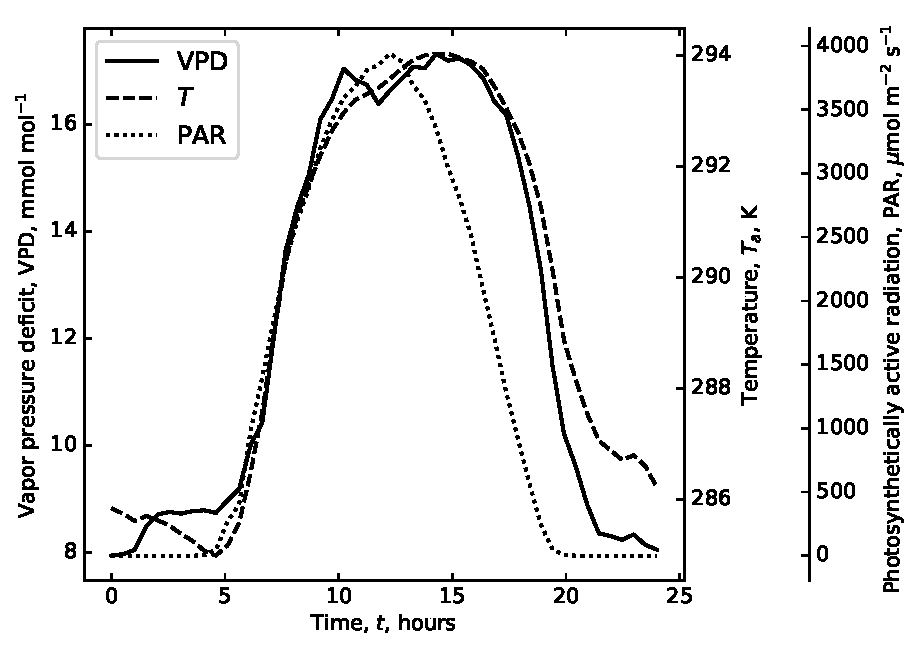
\includegraphics[scale=0.75]{environment.pdf}   
    \end{center}
    \caption{Diurnal trends of vapor pressure deficit (VPD), temperature ($T$), and photosynthetically active radiation (PAR). These are the averaged trends using measurements from the FLUXNET project at the Blodgett forest over 20 days starting from 5-29-2004 (the start of 4-months drought). These trends are repeated for the desired simulation duration.}
    \label{fig:environment}
\end{figure}

\begin{figure}[h]
    \begin{center}
         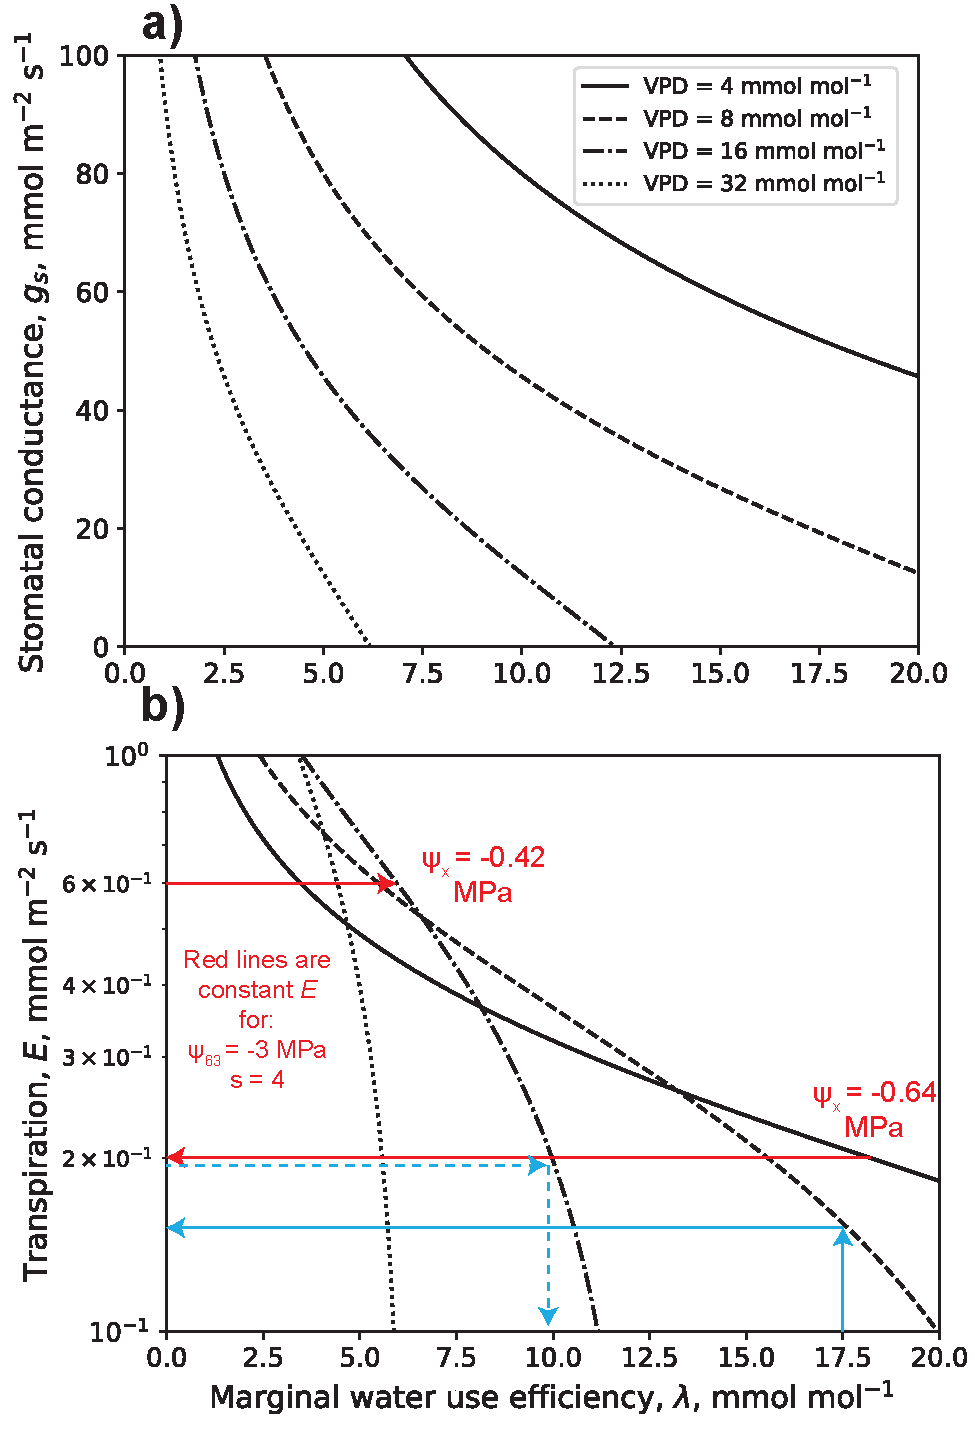
\includegraphics[scale=0.5]{g_E_lam_noon.pdf}   
    \end{center}
    \caption{a) Phase space of stomatal conductance $g_s$ vs the marginal water use efficiency $\lambda$ as a result of equation \ref{eqn:control} for different vapor pressure deficits (VPD). Other environmental conditions correspond to those shown in figure \ref{fig:environment} at noon and in table \ref{tab:props}. An increase in VPD or $\lambda$ both decrease $g_s$ with the other kept at constant. b) Transpiration $E$ corresponding to the curves in the phase space in panel a. An increase in $\lambda$ always leads to a decrease in $E$ when VPD is kept constant however the change in $E$ with changing VPD is more nuanced and depends on the value of $\lambda$. The solid blue arrows show how the value of $\lambda$ determines $E$ when transpiration is demand driven. When transpiration is supply limited, the maximum $E$ possible determines $\lambda$ as illustrated by the dashed blue arrows. Red horizontal arrows show the trends in $\lambda$ with changing VPD for supply limited transpiration of a plant with vulnerability curve (VC) parameters $\psi_{63}=-3$ MPa and $s=4$. The upper red arrow, showing constant $E$ at soil water potential $\psi_x = -0.42$ MPa, shows how $\lambda$ increases as the air dries from VPD$=4$ mmol mol$^{-1}$ to VPD$=16$ mmol mol$^{-1}$. The trend reverses as VPD continues increasing to $32$ mmol mol$^{-1}$. At $\psi_x = -0.64$ MPa, the trend in $\lambda$ reverses as shown by the lower red line. One can then trace these $\lambda$ trends to $g_s$ in panel a and infer magnitudes of midday stomatal closure and day to day $g_s$ sensitivity to drought.}
    \label{fig:gs_E_lam}
\end{figure}

\begin{figure}[h]
    \begin{center}
        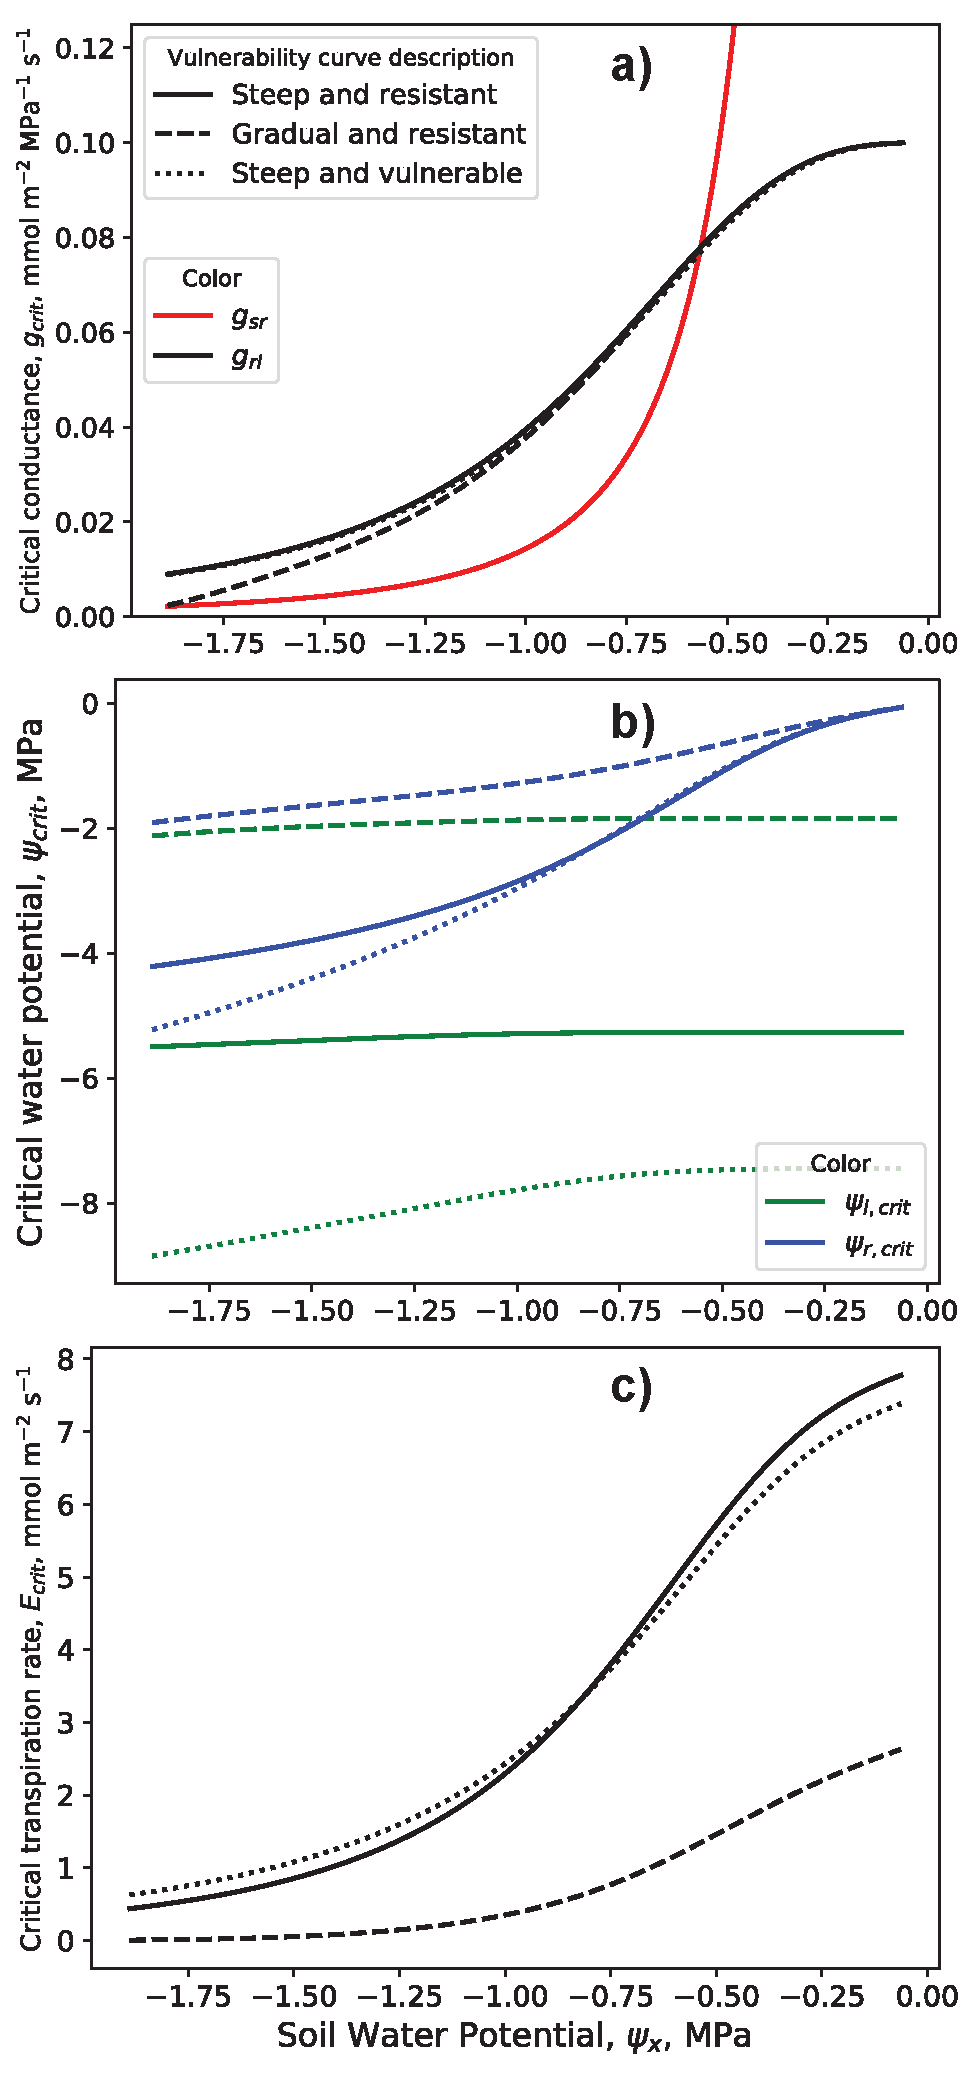
\includegraphics[scale=0.5]{g_psi_E_psix.pdf}
    \end{center}
    \caption{a) Soil to root conductance of the rhizosphere ($g_{sr}$) and root to leaf conductance of the plant ($g_{rl}$) that maximize transpiration $E$ for difference soil water potentials $\psi_x$. Soil is sandy loam and particular hydraulic parameters are shown in table \ref{tab:props}. Three vulnerability curve (VC) examples give different $g_{rl}$ trends. b) Maximizing root and leaf water potential ($\psi_r$ and $\psi_l$, respectively) for the three VCs and for the particular soil type. The exponential VC ($s=1$) can maintain a gap between $\psi_r$ and $\psi_l$ as $\psi_x$ decreases unlike the other two VCs. c) This leads to the exponential VC maintaining a higher $E$ at dry soil and even an order of magnitude larger $E$ compared to the VC with $\psi_{63}=-1.5$ MPa and $s=4$.}
    \label{fig:gmax_Emax_psix}
\end{figure}

\begin{figure}[h]
    \begin{center}
         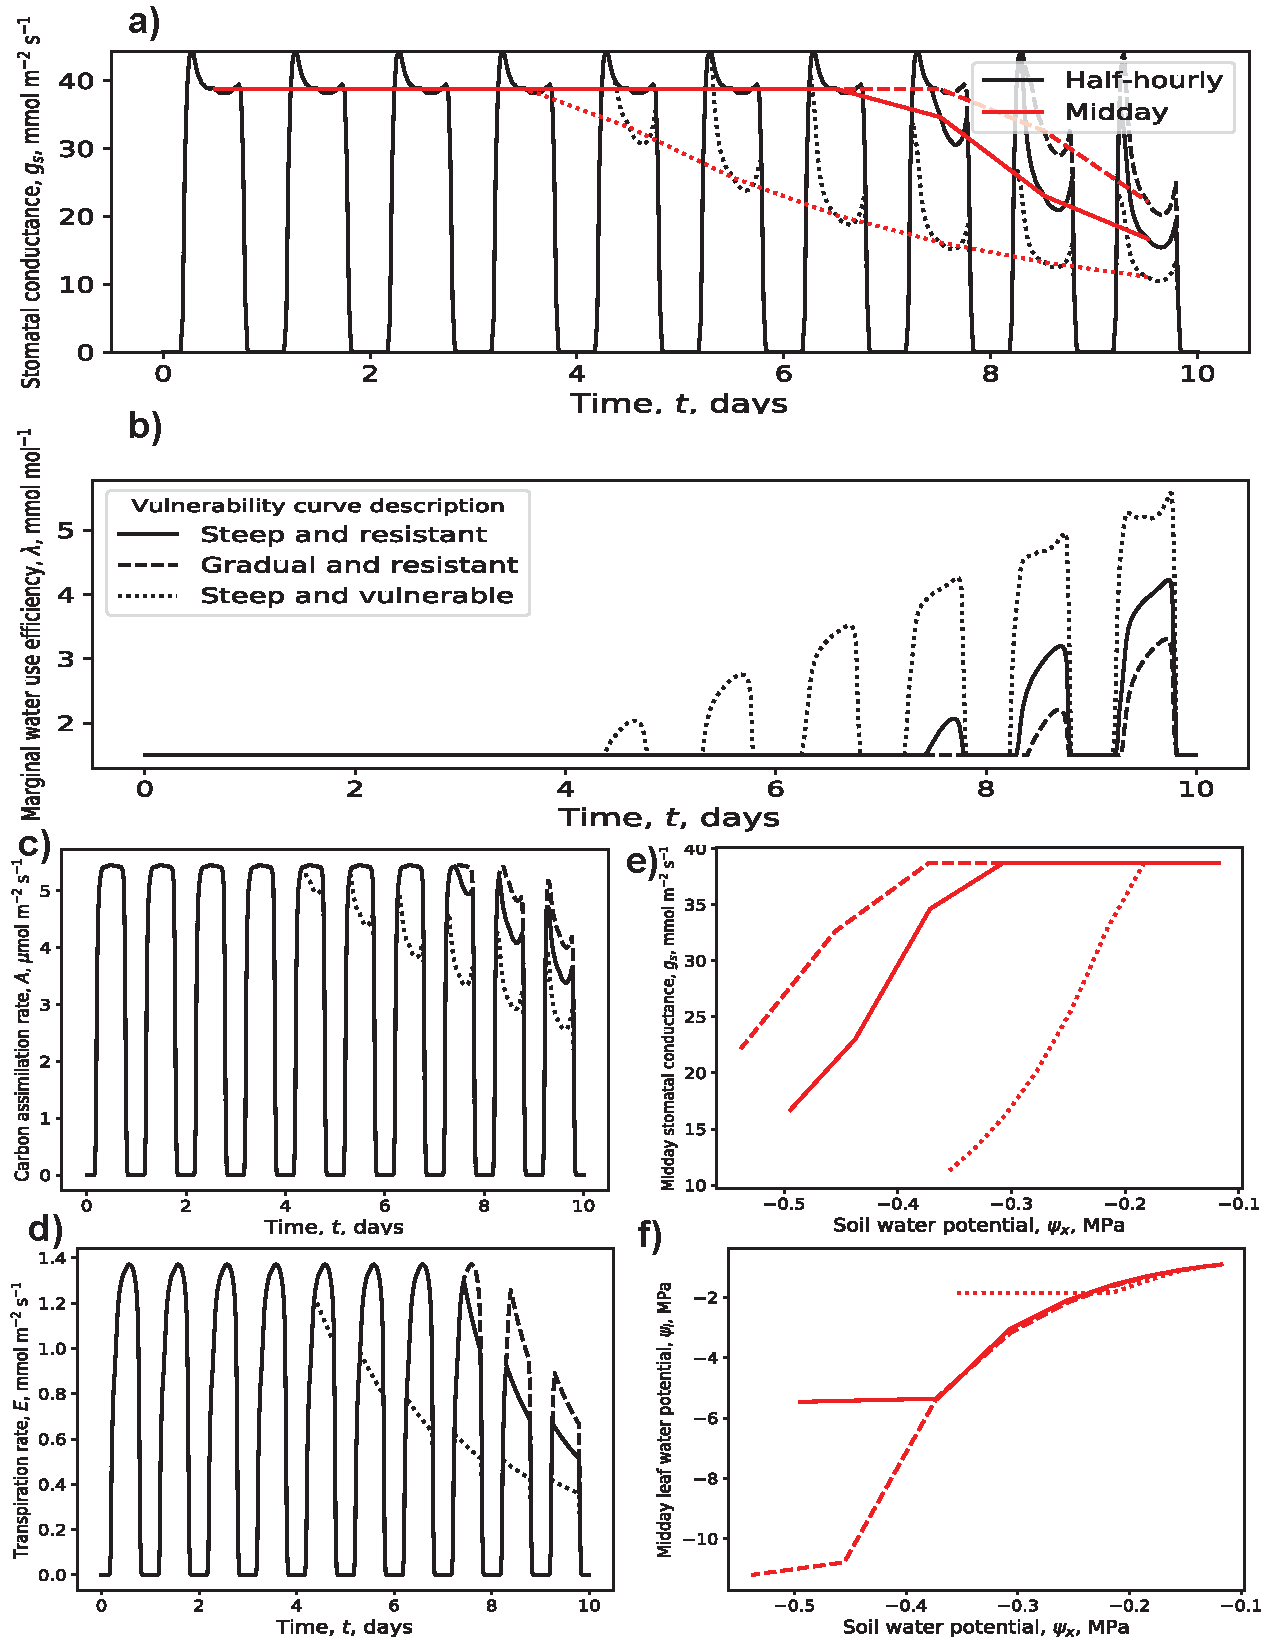
\includegraphics[scale=0.65]{WUS_no_comp.pdf} 
    \end{center}
    \caption{Results of a simulation where at time $t=0$, soil moisture $x(0) =0.22$. There is no competitive soil water users and the terminal marginal water use efficiency is set at $\lambda(10) = 6$ mol mol$^{-1}$. a) Half-hourly (black) and midday (red) trends of stomatal conductance ($g_s$) with $t$ and b) $\lambda$ with $t$. Trends are shown for a resistant plant ($\psi_{63} = -3$ MPa, $s=4$, and $g_{rl,max} = 2$ mmol m$^{-2}$ MPa$^{-1}$ s$^{-1}$), a vulnerable plant ($\psi_{63} = -1.5$ MPa, $s=4$, and $g_{rl,max} = 2$ mmol m$^{-2}$ MPa$^{-1}$ s$^{-1}$), and an exponential vulnerability curve (VC; $\psi_{63} = -1$ MPa, $s=1$, and $g_{rl,max} = 8$ mmol m$^{-2}$ MPa$^{-1}$ s$^{-1}$). Other plant and soil parameters are listed in the appendix. The plant is Pinus radiata and soil is sandy loam. c) Carbon assimilation rate ($A$) and d) transpiration rate ($E$) with $t$. e) Midday $g_s$ and f) Midday leaf water potential $\psi_l$ with soil water potential $\psi_x$.}
    \label{fig:WUS_no_comp}
\end{figure}

\begin{figure}[h]
    \begin{center}
         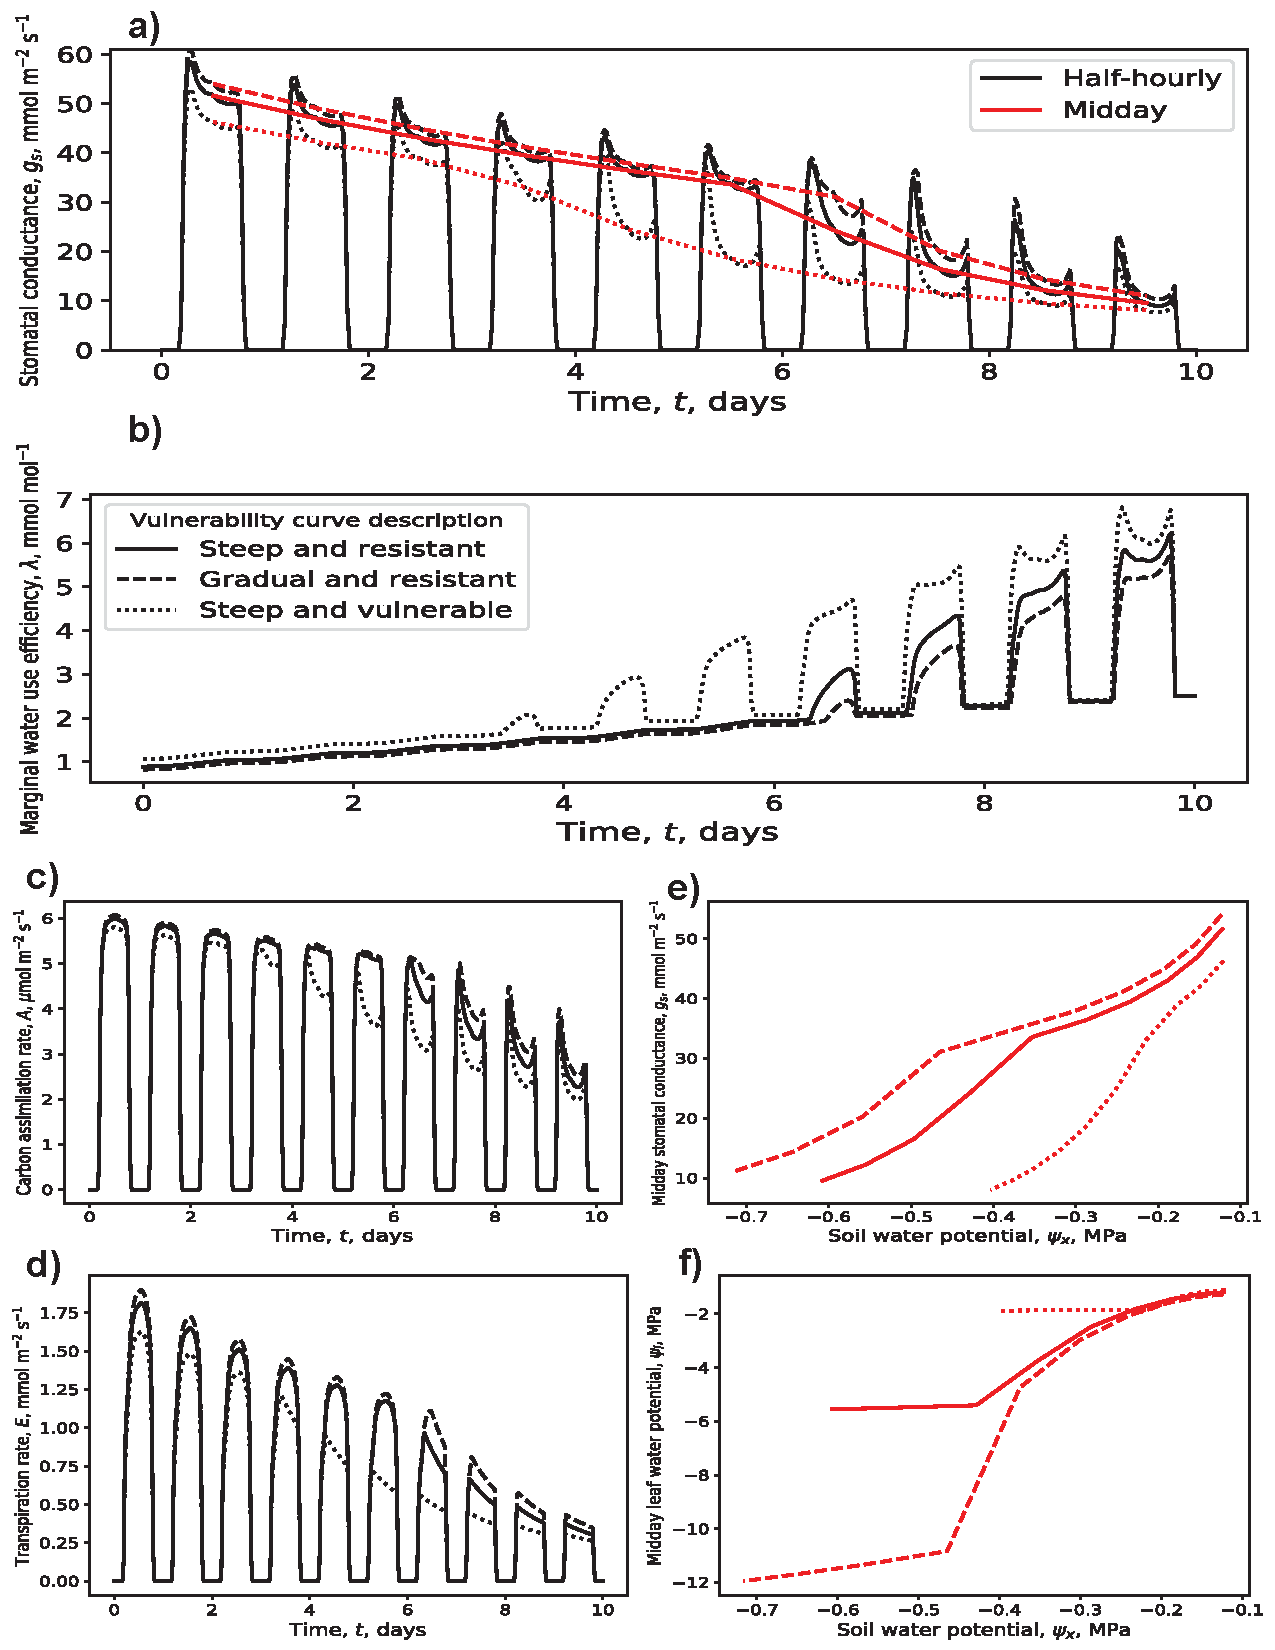
\includegraphics[scale=0.65]{WUS_comp.pdf}   
    \end{center}
    \caption{Results of a simulation where at time $t=0$, soil moisture $x(0) =0.22$. The terminal marginal water use efficiency is set at $\lambda(10) = 8$ mol mol$^{-1}$. The competitive water sinks are soil free drainage and competing plants with similar vulnerability curves (VCs) to those modeled. The competing plants have access to only 20\% of the root zone water of each modeled plant. a) Half-hourly (black) and midday (red) trends of stomatal conductance ($g_s$) with $t$ and b) $\lambda$ with $t$. Trends are shown for a resistant plant ($\psi_{63} = -3$ MPa, $s=4$, and $g_{rl,max} = 2$ mmol m$^{-2}$ MPa$^{-1}$ s$^{-1}$), a vulnerable plant ($\psi_{63} = -1.5$ MPa, $s=4$, and $g_{rl,max} = 2$ mmol m$^{-2}$ MPa$^{-1}$ s$^{-1}$), and an exponential VC ($\psi_{63} = -1$ MPa, $s=1$, and $g_{rl,max} = 8$ mmol m$^{-2}$ MPa$^{-1}$ s$^{-1}$). Other plant and soil parameters are listed in the appendix. The plant is Pinus radiata and soil is sandy loam. c) Carbon assimilation rate ($A$) and d) transpiration rate ($E$) with $t$. e) Midday $g_s$ and f) Midday leaf water potential $\psi_l$ with soil water potential $\psi_x$.}
    \label{fig:WUS_comp}
\end{figure}

\clearpage

%%Figures, tables, and images will be published under a Creative Commons CC-BY licence and permission must be obtained for use of copyrighted material from other sources (including re-published/adapted/modified/partial figures and images from the internet). It is the responsibility of the authors to acquire the licenses, to follow any citation instructions requested by third-party rights holders, and cover any supplementary charges.

\subsection{Tables}
% Tables should be inserted at the end of the manuscript. Please build your table directly in LaTeX.Tables provided as jpeg/tiff files will not be accepted. Please note that very large tables (covering several pages) cannot be included in the final PDF for reasons of space. These tables will be published as \href{http://home.frontiersin.org/about/author-guidelines#SupplementaryMaterial}{Supplementary Material} on the online article page at the time of acceptance. The author will be notified during the typesetting of the final article if this is the case. 


\begin{table}[h]
    \centering
    \begin{tabular}{l l l l}
        Symbol & Description & Value & Unit \\
        \hline
        \multicolumn{4}{l}{}\\
        \multicolumn{4}{l}{\textit{Soil and root properties}}\\
        \hline
        % \multicolumn{4}{l}{}\\
        $\psi_{sat}$ & Saturation water potential & -1.5 & kPa\\
        $\psi_x$ & Soil water potential & & MPa\\
        $x$ & relative soil moisture & & m$^{3}$ m$^{-3}$\\
        $g_{sr,max}$ & Maximum ground area specific soil-root conductance & $0.72 * 10^{-3}$ & kg s m$^{-3}$ \\
        $g_{sr}$ & Ground area specific soil-root conductance & & kg s m$^{-3}$\\
        $b$ & Power law dependence parameter with $\psi_x$ & 3.1 & \\
        $RAI$ & Root area index & $5 \rightarrow 10$ & m$^{2}$ m$^{-2}$\\
        $D_r$ & Average fine root diameter & 1 & mm \\
        $Z_r$ & Average rooting depth & 0.3 & m\\ 
        $U$ & Uncontrolled losses of soil water & & mmol m$^{-2}$ s$^{-1}$\\
        \hline
        \multicolumn{4}{l}{}\\
        \multicolumn{4}{l}{\textit{Above-ground plant properties}}\\
        \hline
        $g_{rl,max}$ & Maximum leaf area specific root-leaf conductance & 2 & mmol m$^{-2}$ s$^{-1}$ MPa$^{-1}$ \\
        $g_{rl}$ & Leaf area specific root-leaf conductance & & mmol m$^{-2}$ s$^{-1}$ MPa$^{-1}$ \\
        $\psi_{63}$ & water potential at which $g_{rl} \approx 0.34 g_{rl,max}$ & $-3 \rightarrow -1$ & MPa \\
        $s$ & Shape parameter of the vulnerability curve & $1 \rightarrow 4$ &  \\
        $g_s$ & Leaf area specific stomatal conductance & & mmol m$^{-2}$ s$^{-1}$ \\
        LAI & Leaf area index & 1.5 & m$^{2}$ m$^{-2}$\\
        \hline
        \multicolumn{4}{l}{}\\
        \multicolumn{4}{l}{\textit{Environmental properties}}\\
        \hline
        VPD & Vapor Pressure Deficit & $4 \rightarrow 32$ & mmol mol$^{-1}$\\
        $T_a$ & Atmospheric temperature & $284 \rightarrow 294$ & K \\
        PAR & Incoming photosynthetically active radiation & $0 \rightarrow 4000$ & $\mu$mol m$^{-2}$ s$^{-1}$ \\
        \hline
        \multicolumn{4}{l}{}\\
        \multicolumn{4}{l}{\textit{Optimization results}}\\
        \hline
        $E$ & Leaf area specific transpiration rate & & mmol m$^{-2}$ s$^{-1}$\\
        $A$ & Leaf area specific carbon assimilation rate & & mmol m$^{-2}$ s$^{-1}$\\
        $\lambda$ & Lagrange multiplier of the soil water balance constraint & & mmol mol$^{-1}$\\
        $L$ & Augmented lagrangian & & mmol m$^{-2}$ s$^{-1}$\\
        $J$ & Objective function to be maximized & & mmol m$^{-2}$\\
        $T$ & Drydown period & 10 & days\\
        $H$ & Hamiltonian & & mmol m$^{-2}$ s$^{-1}$\\
    \end{tabular}
    \caption{Symbols of soil, plant, and environmental properties along with their description, typical values, and units. Values for specific simulations will be mentioned in the simulation description and in the corresponding figure caption.}
    \label{tab:props}
\end{table}


% \section{Nomenclature}

% \subsection{Resource Identification Initiative}
% To take part in the Resource Identification Initiative, please use the corresponding catalog number and RRID in your current manuscript. For more information about the project and for steps on how to search for an RRID, please click \href{http://www.frontiersin.org/files/pdf/letter_to_author.pdf}{here}.

% \subsection{Life Science Identifiers}
% Life Science Identifiers (LSIDs) for ZOOBANK registered names or nomenclatural acts should be listed in the manuscript before the keywords. For more information on LSIDs please see \href{http://www.frontiersin.org/about/AuthorGuidelines#InclusionofZoologicalNomenclature}{Inclusion of Zoological Nomenclature} section of the guidelines.


% \section{Additional Requirements}

% For additional requirements for specific article types and further information please refer to \href{http://www.frontiersin.org/about/AuthorGuidelines#AdditionalRequirements}{Author Guidelines}.

\section*{Conflict of Interest Statement}
%All financial, commercial or other relationships that might be perceived by the academic community as representing a potential conflict of interest must be disclosed. If no such relationship exists, authors will be asked to confirm the following statement: 

The authors declare that the research was conducted in the absence of any commercial or financial relationships that could be construed as a potential conflict of interest.

\section*{Author Contributions}

The Author Contributions section is mandatory for all articles, including articles by sole authors. If an appropriate statement is not provided on submission, a standard one will be inserted during the production process. The Author Contributions statement must describe the contributions of individual authors referred to by their initials and, in doing so, all authors agree to be accountable for the content of the work. Please see  \href{http://home.frontiersin.org/about/author-guidelines#AuthorandContributors}{here} for full authorship criteria.

\section*{Funding}
Details of all funding sources should be provided, including grant numbers if applicable. Please ensure to add all necessary funding information, as after publication this is no longer possible.

\section*{Acknowledgments}
This is a short text to acknowledge the contributions of specific colleagues, institutions, or agencies that aided the efforts of the authors.

\section*{Supplemental Data}
 \href{http://home.frontiersin.org/about/author-guidelines#SupplementaryMaterial}{Supplementary Material} should be uploaded separately on submission, if there are Supplementary Figures, please include the caption in the same file as the figure. LaTeX Supplementary Material templates can be found in the Frontiers LaTeX folder.

\section*{Data Availability Statement}
The datasets [GENERATED/ANALYZED] for this study can be found in the [NAME OF REPOSITORY] [LINK].
% Please see the availability of data guidelines for more information, at https://www.frontiersin.org/about/author-guidelines#AvailabilityofData

\bibliographystyle{frontiersinSCNS_ENG_HUMS} % for Science, Engineering and Humanities and Social Sciences articles, for Humanities and Social Sciences articles please include page numbers in the in-text citations
%\bibliographystyle{frontiersinHLTH&FPHY} % for Health, Physics and Mathematics articles
\bibliography{references}

%%% Make sure to upload the bib file along with the tex file and PDF
%%% Please see the test.bib file for some examples of references

% \section*{Figure captions}

% %%% Please be aware that for original research articles we only permit a combined number of 15 figures and tables, one figure with multiple subfigures will count as only one figure.
% %%% Use this if adding the figures directly in the mansucript, if so, please remember to also upload the files when submitting your article
% %%% There is no need for adding the file termination, as long as you indicate where the file is saved. In the examples below the files (logo1.eps and logos.eps) are in the Frontiers LaTeX folder
% %%% If using *.tif files convert them to .jpg or .png
% %%%  NB logo1.eps is required in the path in order to correctly compile front page header %%%

% \begin{figure}[h!]
% \begin{center}
% 
\includegraphics[width=10cm]{logo1}% This is a *.eps file
% \end{center}
% \caption{ Enter the caption for your figure here.  Repeat as  necessary for each of your figures}\label{fig:1}
% \end{figure}


% \begin{figure}[h!]
% \begin{center}
% \includegraphics[width=15cm]{logos}
% \end{center}
% \caption{This is a figure with sub figures, \textbf{(A)} is one logo, \textbf{(B)} is a different logo.}\label{fig:2}
% \end{figure}

%%% If you are submitting a figure with subfigures please combine these into one image file with part labels integrated.
%%% If you don't add the figures in the LaTeX files, please upload them when submitting the article.
%%% Frontiers will add the figures at the end of the provisional pdf automatically
%%% The use of LaTeX coding to draw Diagrams/Figures/Structures should be avoided. They should be external callouts including graphics.

\end{document}
